  % HB9ARK, 25-SEP-2026 Relaisstation HB9UF auf dem Uetliberg

\documentclass[tikz,border=4pt]{standalone}
\usepackage{tikz}
\usetikzlibrary{arrows.meta}

% Farben: f1 = Eingabe/RX zum Relais (blau), f2 = Ausgabe/TX vom Relais (orange, wie im Original)
\definecolor{rxblau}{rgb}{0.10,0.35,0.75}
\definecolor{txorange}{rgb}{0.8823,0.3137,0.1372}

\begin{document}
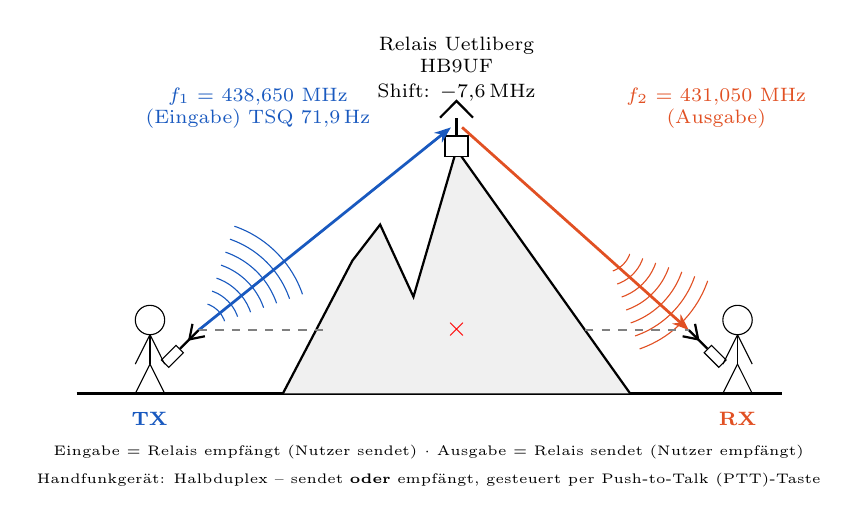
\begin{tikzpicture}[yscale=-1,x=1bp,y=1bp]

  % --- Grundlinie (Boden) ---
  \draw[line width=0.8bp] (0.70,102.79) -- (254.53,102.79);

  % --- Berg als einzelner Kegel (Relais liegt exakt auf der Kuppe) ---
  \fill[gray!12] (75,102.79) -- (100,55) -- (110,42) -- (122,68) -- (137.5,15) -- (200,102.79) -- cycle;
  \draw[line width=0.8bp] (75,102.79) -- (100,55) -- (110,42) -- (122,68) -- (137.5,15) -- (200,102.79);

  % --- Relais-Mast mit kleinem Geraete-Kasten (statt reiner Antennenspitze) ---
  \draw[line width=0.8bp] (137.5,15) -- (137.5,3.5);
  \draw[line width=0.8bp] (131.57,3.5) -- (137.5,-2.5) -- (143.43,3.5);
  \draw[line width=0.6bp,fill=white] (133.25,10) rectangle (141.75,17.5);

  \node[align=center,font=\scriptsize] at (137.5,-14) {Relais Uetliberg\\HB9UF\\[1pt]Shift: $-7{,}6\,$MHz};

  % ======================================================================
  % Linker Standort (Sender): Strichmaennchen + Handfunkgeraet
  % ======================================================================
  \draw[line width=0.4bp] (21.86,102.79) -- (24.50,97.50) -- (27.15,92.22);
  \draw[line width=0.4bp] (32.43,102.79) -- (27.15,92.22);

  \draw[line width=0.4bp] (27.15,92.22) -- (27.15,86.93) -- (27.15,81.64);
  \draw[line width=0.4bp] (27.15,81.64) -- (29.79,86.93) -- (32.43,92.22);
  \draw[line width=0.4bp] (27.15,81.64) -- (21.86,92.22);

  \draw[line width=0.4bp] (27.145,76.352) circle (5.289);

  \draw[line width=0.4bp] (39.141,88.133) -- (36.516,85.508) -- (31.258,90.762) -- (33.887,93.391) -- cycle;

  \draw[line width=0.8bp] (37.969,86.680) -- (44.676,79.973);
  \draw[line width=0.8bp] (42.441,77.734) -- (41.324,83.324) -- (46.914,82.207);
  \node[font=\bfseries\scriptsize,rxblau] at (27,112) {TX};

  % kleiner Wellenfaecher am linken Handfunkgeraet, in RX-Farbe (f1, geht zum Relais)
  \begin{scope}
    \clip (44.676,79.973) -- (59.352,37.344) -- (87.305,65.297) -- cycle;
    \foreach \r in {39.53,34.59,29.65,24.71,19.77,14.82,9.88}
      \draw[line width=0.4bp,rxblau] (44.677,79.972) circle (\r);
  \end{scope}

  % ======================================================================
  % Rechter Standort (Empfaenger): Strichmaennchen + Handfunkgeraet
  % ======================================================================
  \draw[line width=0.4bp] (233.375,102.793) -- (236.019,97.504) -- (238.664,92.219);
  \draw[line width=0.4bp] (243.953,102.793) -- (238.664,92.219);

  \draw[line width=0.4bp] (238.664,92.219) -- (238.664,86.930) -- (238.664,81.641);
  \draw[line width=0.4bp] (238.664,81.641) -- (241.309,86.930) -- (243.953,92.219);
  \draw[line width=0.4bp] (238.664,81.641) -- (233.375,92.219);

  \draw[line width=0.4bp] (238.664,76.352) circle (5.289);

  \draw[line width=0.4bp] (229.293,85.508) -- (226.664,88.133) -- (231.922,93.391) -- (234.551,90.762) -- cycle;

  \draw[line width=0.8bp] (227.840,86.680) -- (221.129,79.973);
  \draw[line width=0.8bp] (218.895,82.207) -- (224.484,83.324) -- (223.367,77.734);
  \node[font=\bfseries\scriptsize,txorange] at (238.7,112) {RX};

  % kleiner Wellenfaecher am rechten Handfunkgeraet, in TX-Farbe (f2, kommt vom Relais)
  \begin{scope}
    \clip (190.535,49.375) -- (233.160,64.051) -- (205.211,92.004) -- cycle;
    \foreach \r in {39.53,34.59,29.65,24.71,19.77,14.82,9.88}
      \draw[line width=0.4bp,txorange] (190.534,49.375) circle (\r);
  \end{scope}

  % ======================================================================
  % Signalpfeile: links -> Relais (Eingabe f1) und Relais -> rechts (Ausgabe f2)
  % Als gerade Linien -- physikalisch korrekt, da sich Funkwellen geradlinig
  % ausbreiten. Da das Relais auf der Kuppe (dem hoechsten Punkt) sitzt,
  % verlaeuft die direkte Sichtlinie von jedem Standort zur Antenne stets
  % oberhalb der Bergflanke.
  % ======================================================================
  \draw[line width=1bp,rxblau,-{Stealth[length=6pt]}]
    (44.676,79.973) -- (135.5,7);

  \draw[line width=1bp,txorange,-{Stealth[length=6pt]}]
    (139.5,7) -- (221.129,79.973);

  % Beschriftung der Frequenzen
  \node[align=center,font=\scriptsize,rxblau] at (66,0) {$f_1$ = 438,650 MHz\\(Eingabe) TSQ 71,9\,Hz};
  \node[align=center,font=\scriptsize,txorange] at (231,0) {$f_2$ = 431,050 MHz\\(Ausgabe)};

  % ======================================================================
  % Blockierte Direktverbindung: ohne Relais kein Sichtkontakt zwischen
  % den beiden Standorten, da der Berg dazwischen liegt.
  % ======================================================================
  \draw[dashed,gray,line width=0.6bp] (44.676,79.973) -- (91.24,79.973);
  \draw[dashed,gray,line width=0.6bp] (183.75,79.973) -- (221.129,79.973);
  \node[font=\bfseries,red] at (137.5,79.973) {$\times$};

  % --- Verknuepfung Relais-Sicht (Eingabe/Ausgabe) mit Nutzer-Sicht (TX/RX) ---
  \node[align=center,font=\tiny] at (127.5,124)
    {Eingabe = Relais empf\"angt (Nutzer sendet) $\cdot$ Ausgabe = Relais sendet (Nutzer empf\"angt)};
  \node[align=center,font=\tiny] at (127.5,134)
    {Handfunkger\"at: Halbduplex -- sendet \textbf{oder} empf\"angt, gesteuert per Push-to-Talk (PTT)-Taste};

\end{tikzpicture}
\end{document}
